\documentclass[12pt]{article}
\usepackage{times} 			% use Times New Roman font

\usepackage[margin=1in]{geometry}   % sets 1 inch margins on all sides
\usepackage{hyperref}               % for URL formatting
\usepackage[pdftex]{graphicx}       % So includegraphics will work
\setlength{\parskip}{1em}           % skip 1em between paragraphs
\usepackage{indentfirst}            % indent the first line of each paragraph
\usepackage{datetime}
\usepackage[small, bf]{caption}
\usepackage{listings}               % for code listings
\usepackage{xcolor}                 % for styling code
\usepackage{multirow}

%New colors defined below
\definecolor{backcolour}{RGB}{246, 246, 246}   % 0xF6, 0xF6, 0xF6
\definecolor{codegreen}{RGB}{16, 124, 2}       % 0x10, 0x7C, 0x02
\definecolor{codepurple}{RGB}{170, 0, 217}     % 0xAA, 0x00, 0xD9
\definecolor{codered}{RGB}{154, 0, 18}         % 0x9A, 0x00, 0x12

%Code listing style named "gcolabstyle" - matches Google Colab
\lstdefinestyle{gcolabstyle}{
  basicstyle=\ttfamily\small,
  backgroundcolor=\color{backcolour},   
  commentstyle=\itshape\color{codegreen},
  keywordstyle=\color{codepurple},
  stringstyle=\color{codered},
  numberstyle=\ttfamily\footnotesize\color{darkgray}, 
  breakatwhitespace=false,         
  breaklines=true,                 
  captionpos=b,                    
  keepspaces=true,                 
  numbers=left,                    
  numbersep=5pt,                  
  showspaces=false,                
  showstringspaces=false,
  showtabs=false,                  
  tabsize=2
}

\lstset{style=gcolabstyle}      %set gcolabstyle code listing

% to make long URIs break nicely
\makeatletter
\g@addto@macro{\UrlBreaks}{\UrlOrds}
\makeatother

% for fancy page headings
\usepackage{fancyhdr}
\setlength{\headheight}{13.6pt} % to remove fancyhdr warning
\pagestyle{fancy}
\fancyhf{}
\rhead{\small \thepage}
\lhead{\small HW2, Tomar}  % EDIT THIS, REPLACE # with HW number
\chead{\small CS 532, Spring 2023} 

%-------------------------------------------------------------------------
\begin{document}

% EDIT THE ITEMS HERE
\begin{centering}
{\large\textbf{HW2 - Web Archiving}}\\ 
Prashant Tomar\\
02/26/2023\\
\end{centering}

%-------------------------------------------------------------------------

% The * after \section just says to not number the sections
\section*{Q1. Collect URIs from Tweets. Extract 1000 unique links from tweets in Twitter.}



\subsection*{Answer}

This Task is divided into multiple steps to get the required output i.e 1000 unique links from tweets in twitter.

\emph{Step 1: Collects English-language tweets that contain links}

The Tweets were already provided by the Professor in json and jsonl Files.


\emph{Step 2: Extract links from the collected tweets}

The following python code will extract all the URIs from the .JSON file and save the output in a output.txt file.

%Python code highlighting
\begin{lstlisting}[language=Python, caption=Extract the URIs from the .JSON file, label=lst:copy]
import json
import re

# Regular expression to match URLs
url_pattern = re.compile(r'http[s]?://(?:[a-zA-Z]|[0-9]|[$-_@.&+]|[!*\(\),]|(?:%[0-9a-fA-F][0-9a-fA-F]))+')

# Open the JSON file containing tweets
with open('tweets-1140.json', 'r', encoding='utf-8') as f:
    # Load the JSON data
    tweet_data = json.load(f)

    # Loop over each tweet in the data
    for tweet in tweet_data:
        # Extract links from the tweet's text
        links = re.findall(url_pattern, tweet['text'])
        # If links were found, write them to the output file
        if links:
            with open('output.txt', 'a', encoding='utf-8') as out_file:
                out_file.write('Tweet: {}\n'.format(tweet['text']))
                out_file.write('Links:\n')
                for link in links:
                    out_file.write('{}\n'.format(link))
                out_file.write('\n')

  
\end{lstlisting}

\emph{Step 3: Extract links from the collected tweets}

The following python code will extract all the URIs from the .JSONL file and save the output in a output.txt file.

%Python code highlighting
\begin{lstlisting}[language=Python, caption=Extract the URIs from the .JSONL file, label=lst:copy]
import json
import re

# Regular expression to match URLs
url_pattern = re.compile(r'http[s]?://(?:[a-zA-Z]|[0-9]|[$-_@.&+]|[!*\(\),]|(?:%[0-9a-fA-F][0-9a-fA-F]))+')

# Open the JSONL file containing tweets
with open('tweets-1545.jsonl', 'r', encoding='utf-8') as f:
    # Loop over each line in the file
    for line in f:
        # Load the JSON data from the line
        tweet_data = json.loads(line)
        # Extract links from the tweet's text
        links = re.findall(url_pattern, tweet_data['text'])
        # If links were found, write them to the output file
        if links:
            with open('output.txt', 'a', encoding='utf-8') as out_file:
                out_file.write('Tweet: {}\n'.format(tweet_data['text']))
                out_file.write('Links:\n')
                for link in links:
                    out_file.write('{}\n'.format(link))
                out_file.write('\n')

  
\end{lstlisting}

\emph{Step 4: Resolve URIs}

The following Python code will resolve the output.txt file and extract the links from that file and store it into separate resolved-urls.txt file

%Python code highlighting
\begin{lstlisting}[language=Python, caption=Resolve the URIs to extract URLs from output.txt, label=lst:copy]
import requests

# read the URLs from the file
with open('output.txt', 'r', encoding='utf-8') as f:
    urls = [line.strip() for line in f.readlines()]

# resolve each URL and save the final target URI in a new file
with open('resolved_urls.txt', 'w') as f:
    for url in urls:
        try:
            response = requests.get(url, allow_redirects=True, timeout=5)
            final_url = response.url
            f.write(final_url + '\n')
        except:
            print('Error resolving URL:', url)
  
\end{lstlisting}




\emph{Step 5: Resolve URIs to the Final target URI and storing the unique URIs to file}

We will be collecting many shortened links (e.g., dlvr.it, bit.ly, buff.ly, etc.), and our goal is to obtain the actual HTTP 200 URI. To accomplish this, I wrote a Python code that redirects the shortened links to their final URI and saves the resolved links in a file. Additionally, we are performing exception handling to eliminate unwanted URIs. The output of the code is a file named "unique_urls.txt" that contains all the unique links that have been resolved.

%Python code highlighting
\begin{lstlisting}[language=Python, caption=Resolve URIs to the unique target URI, label=lst:copy]
unique_uris = set()

with open('resolved_urls.txt', 'r', encoding='utf-8') as f:
    for line in f:
        uri = line.strip()
        if uri not in unique_uris:
            unique_uris.add(uri)

with open('unique_urls.txt', 'w') as f:
    for uri in unique_uris:
        f.write(uri + '\n')
        
\end{lstlisting}

\emph{Step 6: Remove the utm data from the links }

I used a script that extracts the base URL of each link and eliminates any parameters beginning with "utm" to remove the UTM data from the links. This was necessary because I encountered UTM errors when running the script. The output is a list of cleaned URIs, saved in a file named "cleaned-urls.txt".

%Python code highlighting
\begin{lstlisting}[language=Python, caption=Remove utm to resolve URIs to the final target URI, label=lst:copy]
from urllib.parse import urlparse, parse_qs, urlencode, urlunparse

def remove_utm_params(url):
    parsed_url = urlparse(url)
    query_params = dict()
    for key, value in parse_qs(parsed_url.query).items():
        if not key.startswith('utm_'):
            query_params[key] = value
    new_query_string = urlencode(query_params, doseq=True)
    new_parsed_url = parsed_url._replace(query=new_query_string)
    new_url = urlunparse(new_parsed_url)
    return new_url

input_file = open('unique_urls.txt', 'r')
output_file = open('cleaned_urls.txt', 'w')

for line in input_file:
    url = line.strip()
    new_url = remove_utm_params(url)
    output_file.write(new_url + '\n')

input_file.close()
output_file.close()

        
\end{lstlisting}



\subsection*{Discussion:}

Figure \ref{fig:cleaned-urls} shows the collected tweets in cleaned-urls.txt file.

\begin{figure}[h]
    \centering
    % trim and clip are used to crop the image, trim=left bottom right top
    % width sets max width, height will be scaled appropriately
    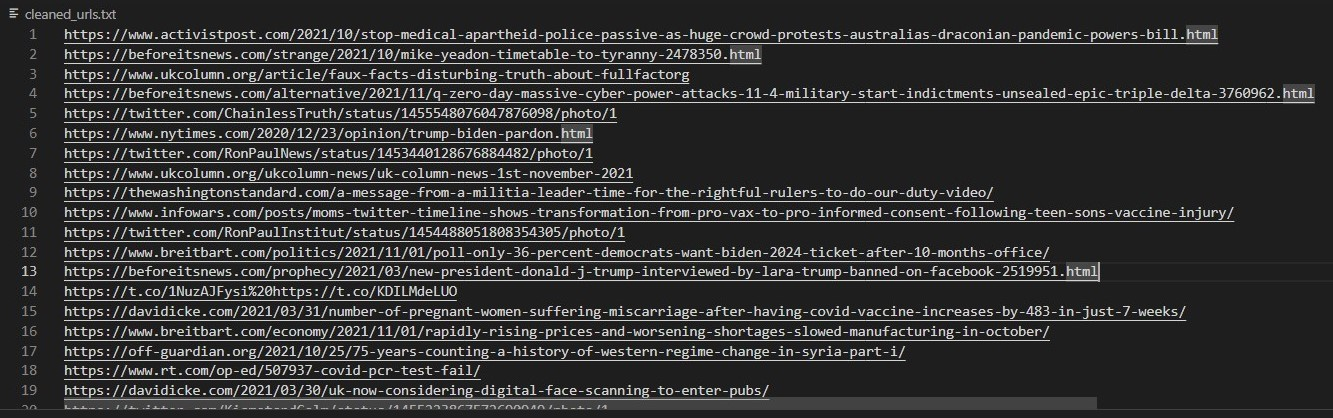
\includegraphics[trim=0 20 10 50, clip, width=\textwidth,height=6cm] {urls.jpg}
    \caption{collection of tweets}
    \label{fig:cleaned-urls}
\end{figure}

To obtain 1000 unique links, we typically need to collect more than 1000 tweets by accessing the Twitter API through a developer account and using the twarc library. However, for this project, the professor has already provided us with the required tweets in the form of JSON and JSONL files, so we don't need to access the Twitter API. As described in step 2 and step 3, I wrote Python code to extract only the tweet URIs while removing any unwanted key-value pairs. However, the extracted URIs included a significant number of shortened links that were not the original links. Therefore, in step 4, I developed Python code to replace all shortened links with their corresponding original links while also handling exceptions for unresolved links and discarding them accordingly.

Finally, the resolved URIs is stored to the file named "cleaned-urls.txt" which consists of more than 1000 unique URIs of tweets.




\section*{Q2. Get TimeMaps for Each URI}

\subsection*{Answer}
I have written the following Python program to obtain the TimeMaps for each of the unique URIs that were generated in Q1 of this report.

%Python code highlighting
\begin{lstlisting}[language=Python, caption=Getting TimeMap for each URIs, label=lst:copy]
import sys
import requests
import os


if not os.path.exists("timemaps"):
    os.mkdir("timemaps")


memento_analysis = open("memento_analysis.txt", "w")

with open("cleaned-urls.txt", "r", encoding='utf-8') as fobj:
    count = 0
    for url in fobj:
        # fname = url.split("/")[2]
        #if not os.path.exists(os.path.join("timemaps")):
            #with open(os.path.join("timemaps", fname), "w") as output_file:
        try:
            response = requests.head("http://localhost:1208/timemap/json/" + url.strip())
            print(f'Writing URL:  {url} : {response.status_code}')
            if response.status_code == 200:
                print(response.headers)
                if "x-memento-count" in response.headers:
                    print(response.headers["x-memento-count"])
                    memento_analysis.write(f'url.strip() : {response.headers["x-memento-count"]}\n')
                #mems = response.content.decode("utf-8")
                #new_timeMaps = mems[2:]
                #output_file.write(mems)
                #output_file.flush()
                count += 1
            print("URLs complete: " + str(count))
        except requests.exceptions.RequestException as e:
            print("Exception: {} for link: {}".format(str(e), url.strip()))

        
\end{lstlisting}

\subsection*{Discussion:}
To obtain TimeMaps for the URIs generated in Q1, we are utilizing Memgator, which is a Memento Aggregator tool. We have extracted each URI from the final links file using a code, and all the final URIs are stored in a file called "cleaned-urls.txt". This file is used to send each URI to the ODU Memento Aggregator, which helps us to obtain the corresponding TimeMaps. Once we obtain the TimeMaps, we save each of them in a file named "memgator-analysis.txt". The output, which includes all the TimeMaps that we aggregated using Memgator in a txt format, is displayed in Figure 2.

Figure \ref{fig:Memento Timemaps} shows the collection of TimeMaps.

\begin{figure}[h]
    \centering
    % trim and clip are used to crop the image, trim=left bottom right top
    % width sets max width, height will be scaled appropriately
    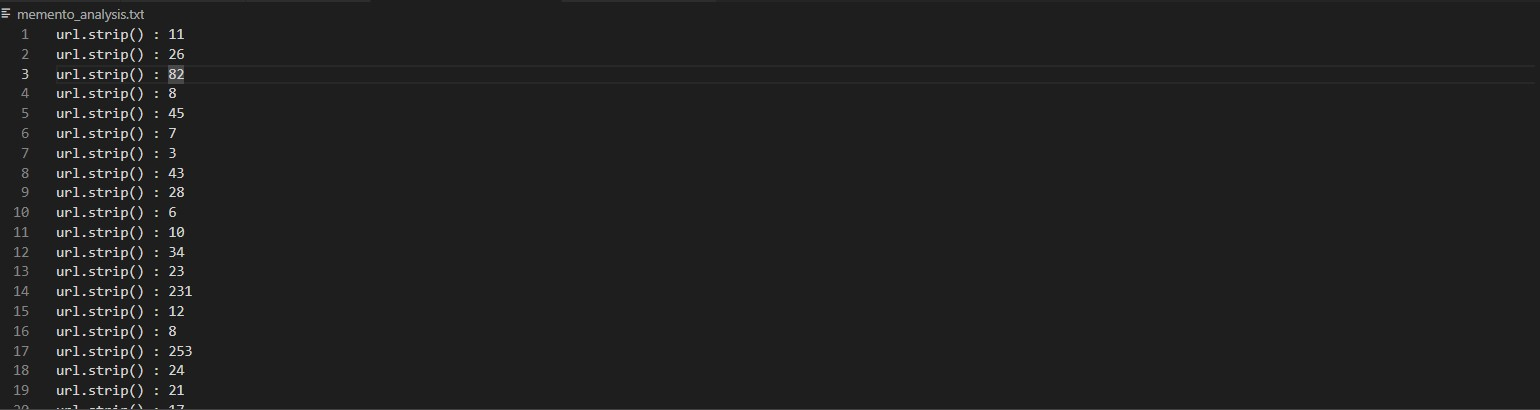
\includegraphics[trim=0 20 10 50, clip, width=\textwidth,height=6cm] {mementos.jpg}
    \caption{collection of tweets}
    \label{fig:Memento Timemaps}
\end{figure}

\section*{Q3 Analyze Mementos Per URI-R}
In the second section of this report, we created separate TimeMaps and stored them in a file named "memento analysis.txt". For URIs with more than zero mementos, we must now determine the memento's count. To do so, I have developed the following code.

%Python code highlighting
\begin{lstlisting}[language=Python, caption=Calculate the mementos by number, label=lst:copy]
with open('memento_analysis.txt') as file:
    data = file.readlines()

# initialize counts for each interval to 0
count_0 = 0
count_1_10 = 0
count_11_20 = 0
count_21_30 = 0
count_31_40 = 0
count_41_50 = 0
count_51_100 = 0
count_101_500 = 0
count_501_1000 = 0
count_1000_plus = 0

# iterate through the list and count numbers in each interval
for number in data:
    number = int(number.strip())  # remove any whitespace and convert to integer
    if number == 0:
        count_0 += 1
    elif number >= 1 and number <= 10:
        count_1_10 += 1
    elif number >= 11 and number <= 20:
        count_11_20 += 1
    elif number >= 21 and number <= 30:
        count_21_30 += 1
    elif number >= 31 and number <= 40:
        count_31_40 += 1
    elif number >= 41 and number <= 50:
        count_41_50 += 1
    elif number >= 51 and number <= 100:
        count_51_100 += 1
    elif number >= 101 and number <= 500:
        count_101_500 += 1
    elif number >= 501 and number <= 1000:
        count_501_1000 += 1
    elif number > 1000:
        count_1000_plus += 1

# print the counts
print("Count of numbers in the list:")
print(f"0: {count_0}")
print(f"1-10: {count_1_10}")
print(f"11-20: {count_11_20}")
print(f"21-30: {count_21_30}")
print(f"31-40: {count_31_40}")
print(f"41-50: {count_41_50}")
print(f"51-100: {count_51_100}")
print(f"101-500: {count_101_500}")
print(f"501-1000: {count_501_1000}")
print(f"1000+: {count_1000_plus}")

        
\end{lstlisting}

\begin{center}
\begin{tabular}{||c c ||} 
 \hline
 Mementos & URI-Rs \\ [0.5ex] 
 \hline\hline
 0-10 & 538  \\ 
 \hline
 11-20 & 198 \\
 \hline
 21-30 & 114  \\
 \hline
 31-40 & 86  \\
  \hline
 41-50 & 28 \\
 \hline
 51-100 & 63  \\
 \hline
 101-500 & 88  \\
 \hline
 501-1000 & 6 \\
 \hline
 Greater than 1000 & 32 \\ [1ex] 
 \hline
\end{tabular}
\end{center}

\subsection*{Discussion}
This is a Python code that reads a list of numbers from a file called 'memento-analysis.txt' and counts how many numbers are in each interval. The code initializes counters for each interval to 0 and iterates through the list of numbers, incrementing the corresponding counter for each interval that the number falls into. Finally, the code prints out the counts for each interval.


\section*{Q5 Explore Conifer and ReplayWeb.Page to archive the Web pages}

\subsection*{Answer}




I opted for the topic of Hyperledger Fabric, a Blockchain framework, to develop a decentralized tool based on private Blockchain. I selected this topic due to my previous years of exploration in the field of Blockchain, where I observed how each release of this framework brings changes in the implementation process of older versions. I encountered no difficulties while archiving the web pages related to this topic, as all the archived pages appeared nearly identical to the original ones.A total of 764 URLs have been archived, with 12 pages archived in their actual page format. The remaining archived URLs are in the format of their implementation mode, such as image files, JSON files, HTML files, and other extensions. I didn't expected the Images count will be the highest among all others file-types. 

Browser link where the WARC file is being located: \url{https://replayweb.page/?source=file%3A%2F%2Fhw2-20230228054045.warc#view=resources&urlSearchType=prefix}

Figure \ref{fig:Conifer} shows the number of pages archived using WARC file.

\begin{figure}[h]
    \centering
    % trim and clip are used to crop the image, trim=left bottom right top
    % width sets max width, height will be scaled appropriately
    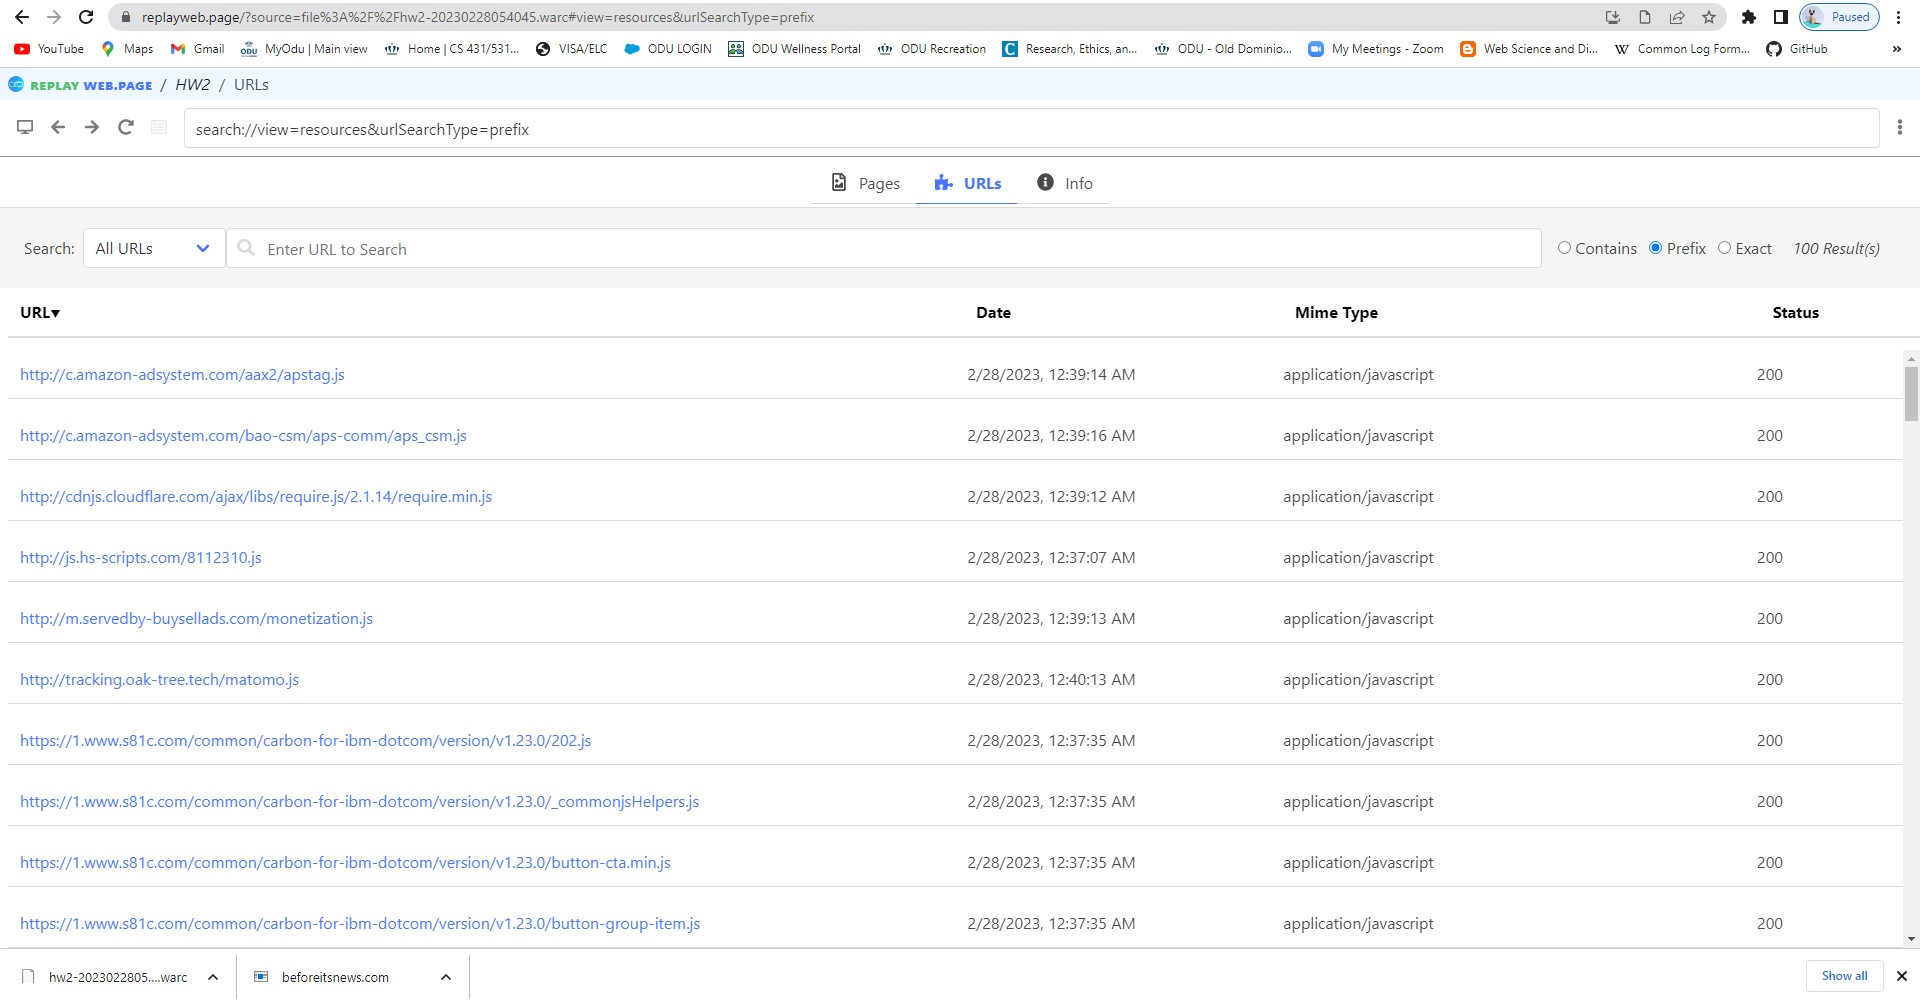
\includegraphics[trim=0 0 0 0, clip, width=\textwidth,height=8cm] {replay-web.jpg}
    \caption{Number of pages archived using WARC file}
    \label{fig:Conifer}
 \end{figure}
 
Figure \ref{fig:archived url} shows the Bar chart created which describes the count of each file type which is been archived.

\begin{figure}[!b]
    \centering
    % trim and clip are used to crop the image, trim=left bottom right top
    % width sets max width, height will be scaled appropriately
    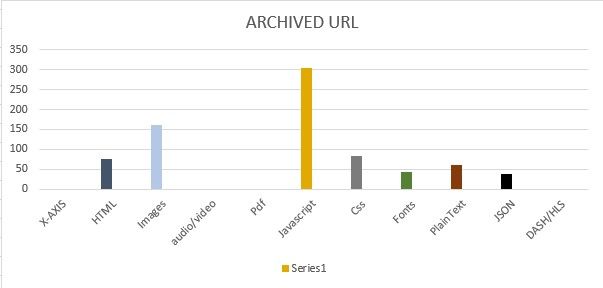
\includegraphics[trim=0 0 0 0, clip, width=\textwidth,height=8cm] {ARCHIVED-URL.JPG}
    \caption{count of each file type being archived}
    \label{fig:archived url}
\end{figure}


A total of 764 URLs have been archived, with 12 pages archived in their actual page format. The remaining archived URLs are in the format of their implementation mode, such as image files, JSON files, HTML files, and other extensions. I didn't expected the Images count will be the highest among all others file-types. 


\section*{References}
\emph Following are the references which I used while doing my HW2, you can refer to some of links from where I took help.

\begin{itemize}
    \item {MemGator, \url{https://github.com/oduwsdl/MemGator}}
    \item {TimeMaps, \url{http://www.mementoweb.org/guide/quick-intro/}}
    \item {Conifer, \url{https://conifer.rhizome.org/}}
    \item {Python requests, \url{https://docs.python-requests.org/en/master/}}
\end{itemize}

\end{document}

